%--------------------------------------------------------------------------------
% ** Second Chapter: Theory
\chapter{Theoretical Background} \label{chap:2}
This chapter .... \textbf{NOT DONE}
\section{Wireless Coexistence Testing}

Wireless coexistence testing is defined as the method of measuring the ability of multiple devices to interact in a single environment with limited bandwidth. It ensures that one device is not impacting other wireless devices operating in the same band. Radio Frequency (RF) regulatory testing is done to demonstrate that the products will use the radio spectrum effectively and comply with local or regional requirements. 

Since the number of interconnected wireless devices operating in 2.4 GHz and 5 GHz ISM (Industrial, Scientific and Medical) band is increasing, it became necessary to control the use of these bands. For this reason, several regulations and local and regional standards are suggested worldwide. Automated test systems to check the compliance of devices with the standards became highly recommended. The quality of coexistence is characterized by the frequency separation, the distance, space and time separation between different users. As big is this separation as much as the Signal to Interference Ratio (SIR) increases. Fundamental coexistence testing approaches can be categorized as conducted testing, radiated controlled environment (e.g. anechoic chambers), or radiated open environment. Some test method may combine all the categories.
Since conducted test methods make use of a configuration of RF cables, combiners or couplers in order to establish communication channels between the various wireless transceivers, this category is easy to setup and usually results in lower measurement uncertainty.
Radiated controlled environments use non-reflective chambers such as anechoic chambers in order to achieve a calibrated field at the location of the DUT. This category is beneficial since the DUTs nowadays do not necessarily come with cable connectors. In addition the radiated measurements exploit the antenna impacts (antenna pattern, efficiency, mismatch) in the measurement which is not possible in conducted measurements.

The approach considered in this work is based on Rohde $\&$ Schwarz TS8997 regulatory test system for wireless coexistence testing. This system already includes vector signal generator, spectrum analyzer and switching modules which is required to perform conducted measurements for regulatory tests mentioned in ETSI and FCC standards. This work investigates the approach of radiated measurements, introduced as TS8997 Regulatory Test System,  uses an RF shielded box (R$\&$S TS7124M) equipped with probe antennas. The approach is described in detail in the later chapters.




Some of the major regulatory bodies that have authority over many technology regulations around the world are the Federal Communications Commission (FCC) and the European Telecommunications Standards Institute (ETSI). This work focuses on tests conform to the criterias and test methodologies mentioned in the standards:
\begin{itemize}
	\item ETSI EN 300 328 V2.2.2 (2019-07): Wideband transmission systems. Data transmission equipment operating in the 2,4 GHz band; Harmonized Standard for access to radio spectrum.

	\item ETSI EN 301 893 V2.1.1 (2017-05) 5 GHz RLAN; Harmonized Standard covering the essential requirements of article 3.2 of Directive 2014/53/EU.
\end{itemize}



In this project, V2.1.1 of the mentioned ETSI standards is the reference to the implemented methodologies. There are about 7 to 8 tests per standard. However, due to the high amount of test cases, a specialized test system and special automated test procedures are of an advantage. The test cases that are explained and implemented in the following chapters for the investigation of the normalized measurements are:
\begin{itemize}
    \item Receiver Blocking
    \item Power Spectral Density
\end{itemize}

Spurious measurements is not supported because normalization is done only for the in band frequencies of the used antennas and thus gain of antenna is not known. In order to perform these measurements, out of band calibration needs to be done for the test chamber. We define following in band test cases:\\

\begin{enumerate}
\item Receiver Blocking (Rx measurement) is a measure of the capability of the equipment to receive a wanted signal on its operating channel without exceeding a given degradation due to the presence of an unwanted input signal (blocking signal) on frequencies other than those of the operating bands provided in the standard. The minimum performance criterion is defined to be a Packet Error Rate (PER) of less than or equal to 10 \%.




\item Power Spectral Density (PSD) is the mean Equivalent Isotropically Radiated Power (EIRP) spectral density in a 1 MHz bandwidth during a transmission burst. The limits depend on the specification of the DUT. The limits are taken from the reference standards.\\
Both test cases and the needed steps are explained in a later chapter.
\end{enumerate}

\section{Antenna Fundamentals}

For this work, a close understanding of the theory of the used antennas and their radiations is needed in order to explain and analyze the physics happening inside of the test system and influencing the measurements in the chamber. This is a main step for further investigations about the quality of the novel normalized wireless measurement approach inside of the test chamber . To describe the performance of antennas, the definition of various parameters is necessary. In the following some of these parameters are highlighted.




\subsection{Radiation Patterns}

One trace of the electric or magnetic field of a considered type of antenna at a constant radius is called the amplitude field pattern. In addition, the spatial variation of the power density along a constant radius can be studied on a graph called the amplitude power pattern. The field and power patterns are usually normalized with respect to their maximum value, yielding normalized field and power patterns. In order to accentuate more the details of the pattern with very low values, usually referred to as minor lobe (photo)the power pattern plot is computed on a logarithmic scale or more commonly in decibels (dB).

A radiation pattern represents the three-dimensional variation of the power radiated by an antenna as a function of the direction away from the antenna. In most cases, the radiation pattern is determined in the far field region and is represented as a function of the directional coordinates (fig. \ref{spherical}). Radiation properties include power flux density, radiation intensity, field strength, directivity, phase or polarization (reference balanis + photos) Different antennas can be classified depending on the characteristics of their patterns. A pattern is called isotropic if the radiation is the same in all directions, which is not realizable in practice but useful for comparison to real antennas. Some antennas may also be described as omnidirectional, which means that the radiation pattern is isotropic in one single plane (photo)for example the dipole antenna and the slot antenna. The third category of antennas is the directional antennas, also called beam antennas The peak represents the direction where the bulk of the radiated power travels. Directional antennas are very common, examples of antennas with highly directional radiation patterns include the  dish antenna and the slotted waveguide antenna. The measurements achieved in this work use six R$\&$ S Vivaldi antennas as probe antennas, and a dipole single-antenna DUT and an omni-directional multi-antenna DUT (photo).

While the radiation pattern is actually three-dimensional, it is common however to describe this behavior with two planar patterns, also called the principal plane patterns (photo). The horizontal pattern, which describes the field strength as a function of the azimuth angle \textit{$ \phi $ } with a fixed elevation angle \textit{$ \vartheta $ }. And the vertical pattern, which describes the field strength as a function of the elecation angle \textit{$ \vartheta $ } for a fixed azimuth angle \textit{$ \phi $ }. These patterns are commonly referred to as azimuth pattern and elevation pattern. The term azimuth describes the reference to the horizontal while the term elevation describes the reference to the vertical. Also, spherical coordinates as shown in Figure 10 are commonly used to describe a location in the three-dimensional space (photo).

%%%%%%%%%%%%%%%%%%%% Figure Spherical %%%%%%%%%%%%%%%%%%%%
\begin{figure}[H]
\centering
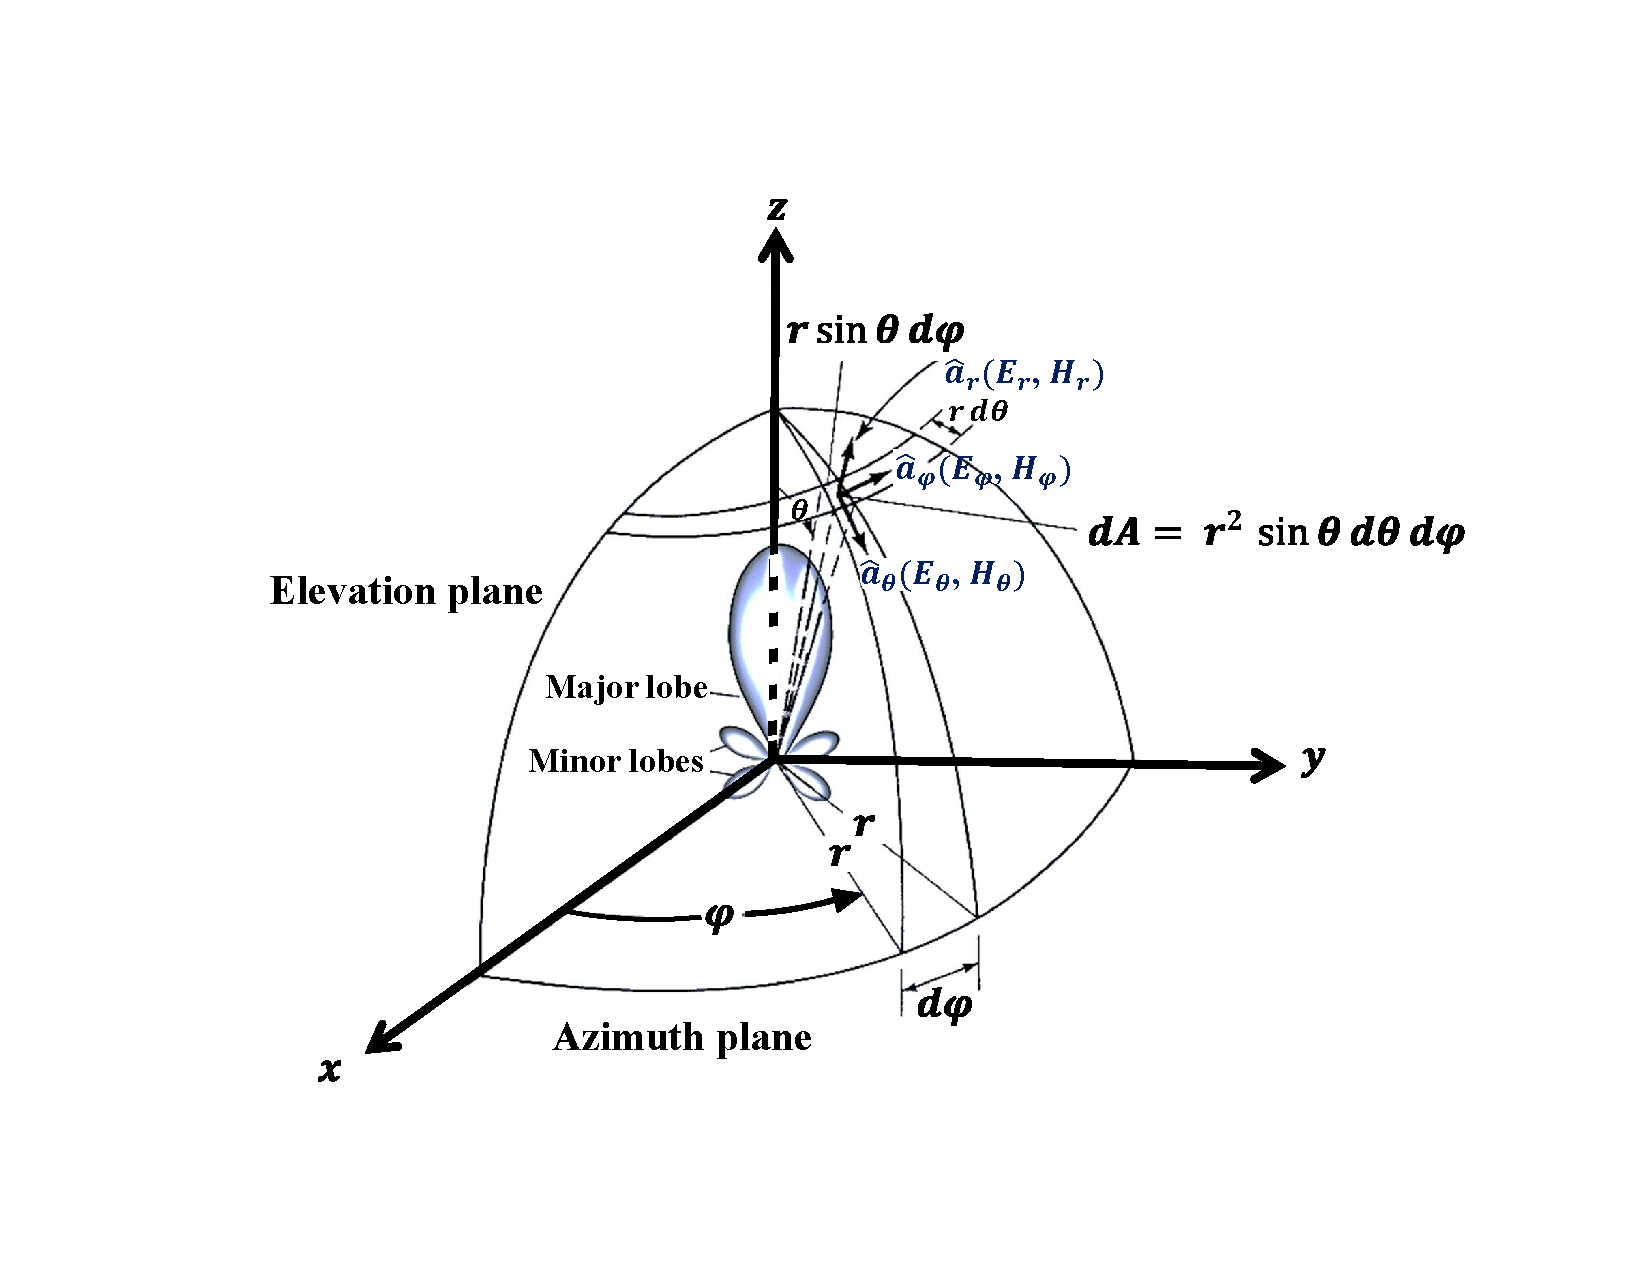
\includegraphics[width=0.6\textwidth]{spherical.pdf}
\caption{spherical coordinates for antena analysis}
\label{fig:resP}
\end{figure}

\begin{figure}
	\begin{center}
		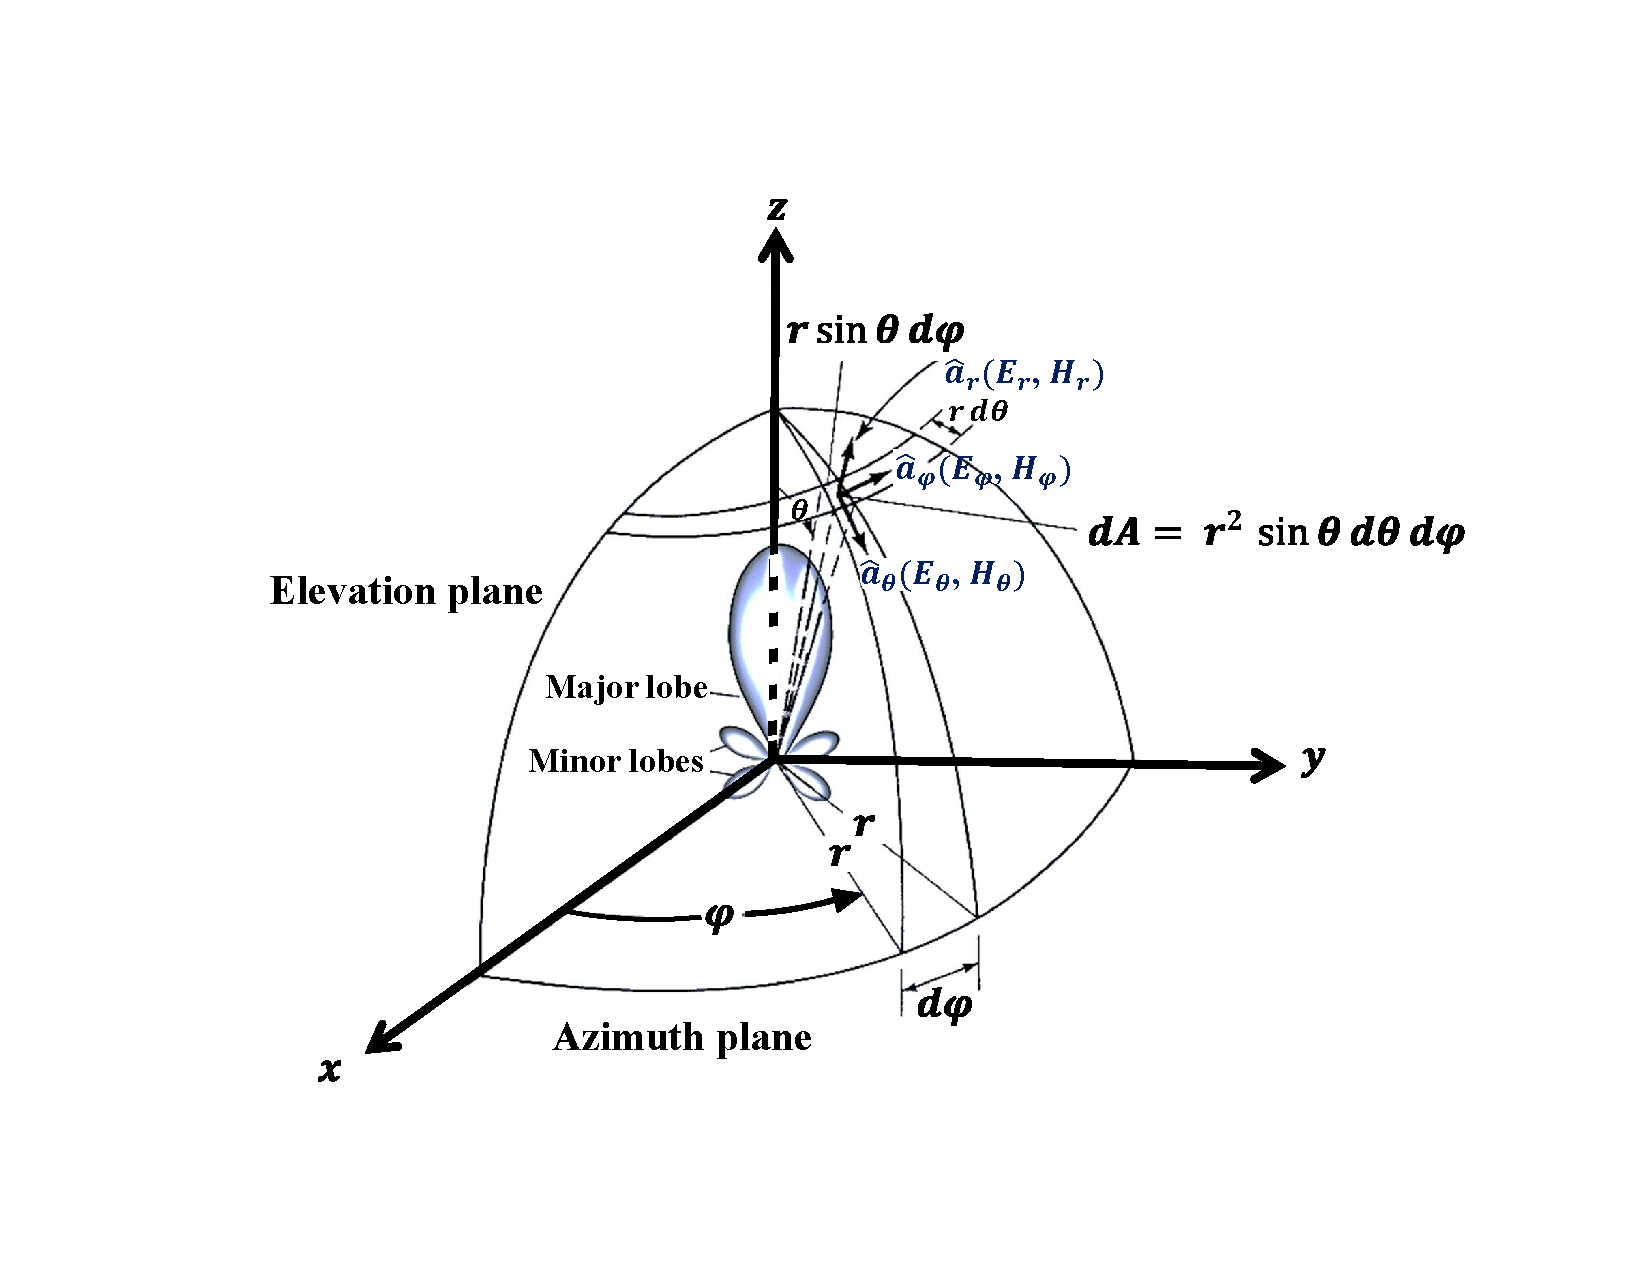
\includegraphics[width=4.92in,height=3.09in]{spherical.pdf}
				\caption{\label{spherical}Spherical coordinates for antena analysis \cite{balanis}}
	\end{center}

\end{figure}


\subsection{Directivity}

Isotropic antennas are theoretical point sources that spread electromagnetic energy equally in all directions. The total radiated power is determined by integrating the power flux density over the surface of a sphere of radius r that surrounds the antenna. The integral represents the theoretical total radiated power. As the distance from the source increases, the surface area of the integrating sphere increases in proportion to the square of the radius of the sphere. The energy from isotropic emitters spreads out evenly to cover this increasingly larger area, and thus the electromagnetic power flux density decreases in proportion to the square of the distance from the source.
The directivity  $D$  of an antenna is the maximal value of its directive gain. Directive gain is represented as  $D \left(  \theta , \varphi  \right)$  and compares the radiant intensity  $U \left(  \theta , \varphi  \right)$  defined as the power per unit solid angle that an antenna creates in a particular direction against the average value over all directions:

$~D \left(  \theta , \varphi  \right) = \frac{ U \left(  \theta , \varphi  \right) }{P_{tot}/ \left( 4 \pi  \right) }$ with $P_{tot}= \int_{ \varphi =}^{ \varphi =2 \pi } \int_{ \theta =0}^{ \theta = \pi }U\sin  \theta d \theta d \varphi $

Directivity is defined as the maximal directive gain value found among all possible solid angles, it is then the ratio of the power density of the physical antenna in its most concentrated direction to that of a theoretical isotropic emitter of the same total power transmission level. Since the directivity is a measure that describes only the directional properties of the antenna, controlled only by the pattern. For example, an antenna that radiated equally well in all directions would have a directivity of 1 (0 dB).



$ D_{0}=max \left( \frac{~U \left(  \theta , \varphi  \right) }{\frac{P_{tot}}{4 \pi }} \right) ~=\frac{~  U \left(  \theta , \varphi  \right)  \vert_{\max }}{\frac{1}{4 \pi } \int_{0}^{2 \pi } \int _{0}^{ \pi }U \left(  \theta , \varphi  \right) \sin  \theta d \theta d \varphi } $


%%%%%%%%%%%%%%%%%%%% Figure 2Dpattern %%%%%%%%%%%%%%%%%%%%





\subsection{Efficiency}

The total antenna efficiency considers losses at the input terminals and within the structure of the antenna. The total efficiency of an antenna is the radiation efficiency multiplied by the impedance mismatch loss of the antenna, when connected to a transmission line or receiver so that the total efficiency can be computed as:

\begin{center}
$ e_{total}= e_{ref}e_{cd}= e_{cd} \left( 1- \vert  \Gamma  \vert ^{2} \right)  $.
\end{center}

Where e\textsubscript{total} is the total efficiency, e\textsubscript{ref} is the reflection or mismatch efficiency, e\textsubscript{cd }is the radiation efficiency which is the product of the conduction efficiency and the dielectric efficiency. This antenna radiation efficiency quantifies the actual losses of a particular antenna design due to many factors such as manufacturing faults, impedance mismatch, surface coating losses, or other factors. It is computed as the ratio of the radiated power to the input power of the antenna and its value lies between 0 and 1 or as a percentage. $\Gamma$ is the voltage reflection coefficient at the input terminals of the antenna:  $\Gamma =\frac{ \left( Z_{in~}- Z_{0~} \right) }{ \left( Z_{in~}+ Z_{0~} \right) }$\  where  $Z_{in~}$ is the antenna’s input impedance and  $Z_{0~}$ is the characteristic impedance of the transmission line, The radiation efficiency, defined as the product of the conduction and the reflection mismatch is later mentioned again to relate the directivity with the gain. An antenna with a high total efficiency has most of the power present at the antenna's input radiated away. A low efficiency antenna has most of the power absorbed as losses within the antenna, or reflected away due to impedance mismatch.

\subsection{Gain}

The antenna gain describes how much power is transmitted in the direction of peak radiation to that of an isotropic source. If the antenna is supposed to have for example 3dB gain, this means that the received power should be 3dB higher than the power that is received at the same input power by an isotropic antenna.


Antenna gain incorporates both directivity and antenna’s efficiency so that the gain is computed as the product of both values. As a result, while directivity is always greater than or equal to 1 (0 dB), antenna gain can be less than 1 (0 dB): 

\begin{center}
$G \left(  \theta , \varphi  \right) =e_{cd} \left[ \frac{~U \left(  \theta , \varphi  \right) }{\frac{P_{tot}}{4 \pi }} \right]$  
\end{center}  


\subsection{Field Regions}

The space around an antenna is usually subdivided into three regions, reactive near-field region, radiating near-field also called Fresnel region and far-field also called Fraunhofer region as seen in figure \ref{field regions} shows changes of antenna amplitude pattern shape in the different field regions.

The closest region to an antenna, with dimensions defined as following: $d \ll $ $ \lambda $ $d \ll $ $ \lambda $ , is termed the near field and is dominated by magnetic fields. A transition zone exists for one to two wavelengths, and then there is the far-field region of an antenna, for which the dimensions are: $d>2\lambda $  , where the electric field becomes dominant.

In far field RF link the ratio between the received and transmitted power can be defined as \textcolor[HTML]{A6A6A6}{(reference):}

$\frac{P_{Rx}}{P_{Tx}}=\frac{G_{Tx}G_{Rx}}{4 \left( kr \right) ^{2}}=\frac{G_{Tx}A_{Rx}}{4 \pi r^{2}}=\frac{A_{Tx}A_{Rx}}{ \lambda ^{2}r^{2}} $


The effective area A, also called aperture of an antenna, is related to gain as follows:  $ A=\frac{ \lambda ^{2}G}{4 \pi } $.

In the near-field, the formula diverges into two different formulas, one for links that are the same (like), either both magnetic or both electric, and one different formula that describes different links (unlike) (reference + figure). In the experiments in this work we only consider electric antennas (like). The ratio is than expressed as following:


 $\frac{P_{Rx}}{P_{Tx}}=\frac{G_{Tx}G_{Rx}}{4} \begin{array}{c}
	 \left( \frac{1}{ \left( kr \right) ^{6}}-\frac{1}{ \left( kr \right) ^{4}}+\frac{1}{ \left( kr \right) ^{2}} \right) ~like~\\
	 \left( \frac{1}{ \left( kr \right) ^{4}}+\frac{1}{ \left( kr \right) ^{2}} \right) ~unlike\\
	\end{array}  $


%%%%%%%%%%%%%%%%%%%% Figure/Image No: 4 starts here %%%%%%%%%%%%%%%%%%%%
%
%\begin{figure}[H]
%	\begin{Center}
%		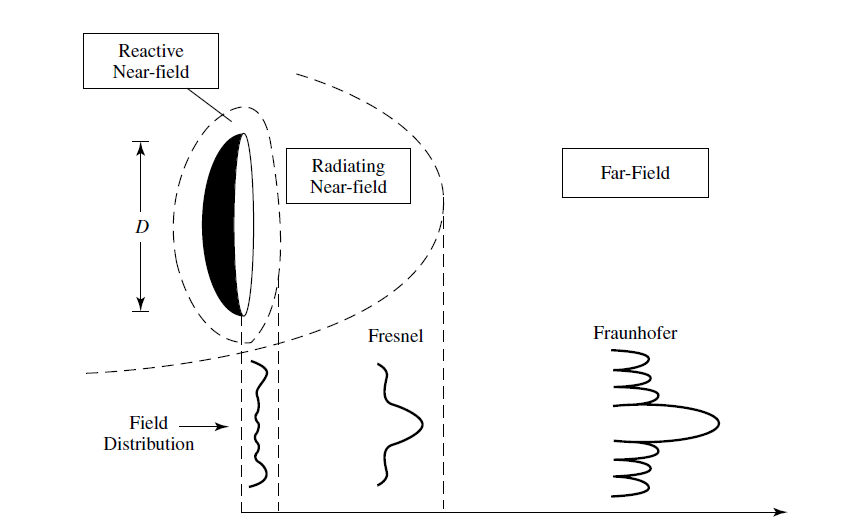
\includegraphics[width=4.43in,height=2.7in]{./media/image4.png}
%		\caption{\label{regions} Field regions of an antenna \cite{}}
%	\end{Center}
%\end{figure}


%%%%%%%%%%%%%%%%%%%% Figure/Image No: 4 Ends here %%%%%%%%%%%%%%%%%%%%


\subsection{Free-space Path Loss}

When there is an unobstructed direct line of-sight path between the antennas for transmitting and receiving, it is possible to estimate the received signal and the link budget. The characterization of the average path loss experienced in a wireless channel helps

to estimate the received signal. The average path loss is defined as$"$  the amount of loss experienced in a propagation

environment as a function of the transmitter-receiver distance$"$  \textcolor[HTML]{A6A6A6}{(reference). }The received

power for free-space propagation can be expressed by the Friis free space equation (reference) expressed by the following formula:

$P_{r} \left( d \right) = P_{t}\frac{G_{t}G_{r} \lambda ^{2}}{ \left( 4 \pi  \right) ^{2}d^{2}} $, where d is the separation distance between the antennas,  $P_{t}$ is the transmitter power, $P_{r}$ is the received power as a function of the distance,  $G_{t}$ the transmitter antenna gain,  $G_{r}$the receiver antenna gain and  $\lambda$ the signal's wavelength in meters.


The path loss which represents the signal attenuation is the ratio between the transmitted power and the received power and are usually measured in dB. The path loss in free-space in dB is given as the following sum, this formula means that higher separation and higher frequency result in higher attenuation:


\subsection{EIRP}

Effective Isotropic Radiated Power (EIRP) is the measured radiated power in a single direction for a fixed angle, so that for antenna radiation pattern measurement the EIRP is considered the maximum value over all measured angles.\\
Based on measurements the EIRP can be computed as following, using the out power at the transmitter $P_{t}$ (in dBm), the cable signal loss $Loss_{c}$ caused by the cable from the transmitter circuit to the antenna and possibly including antenna mismatch (in dB) and the antenna gain $Gain_{a}$ (in dBi):

$EIRP= P_{t} - Loss_{c}+  Gain_{a}$ 


\subsection{Polarization and polarization mismatch}

 The direction of oscillation of the electric field component of an electromagnetic wave describes the polarization of an antenna, when a radio wave is propagating in a medium, is called the polarization of the radio wave. Linear polarization means that the electric field’s vector remains on the same plane all the time, it is considered a special case of elliptical polarization. There are horizontally or vertically polarized radiations, for example omnidirectional are always vertically polarized. Circular polarization means that the electric field’s vector is rotating circularly about the direction of propagation for each RF cycle. The polarization is a design choice during the RF system design.


The difference between the polarization of the receiving antenna and the polarization of the incident wave result in the polarization mismatch, also characterized by the polarization loss factor ( $PLF$) or the polarization efficiency which is the loss of the electromagnetic power due to this polarization mismatch. When receiver’s and transmitters antennas are not aligned\textcolor[HTML]{BFBFBF}{ }there will be a reduction in power transfer between the two antennas and the amount of extracted power from the incoming signal will not be at its maximum. The $PLF$ has a maximum of 1 ( $\text{0 dB}$ ) which means there is no polarization loss and that the receiver antenna receives all the intended incident power of the wave. While a $PLF$ of 0 ( $ -\infty dB$) means that there is a total polarization loss and the antenna at the receiver is unable to capture the incident power. Thus  $0<PLF<1$. In order to calculate the  \( PLF \)  we first look at the far zone of the transmitting antenna, and consider its transmitted electromagnetic field by its components in the transmitter's local spherical coordinate system. The direction of the field is specified by the azimuth and elevation of the receiving antenna in the transmitter's local coordinate system. So that the polarization of the transmitter's antennas may be expressed as following:

$E_{i}= E_{i,H}\hat{e}_{az}+ E_{i,V}\hat{e}_{el}= \widehat{ \rho _{w}}E_{i}$


Where  $E_{i,H}$ and  $E_{i,V}$  are the horizontal and vertical components and  $\widehat{ \rho _{w}}$ is the unit vector of the incident wave. Equivalently, we express the polarization of the receiving antennas with respect to the spherical basis vectors at the receiver's local coordinate system:  $E_{r}= E_{r,H}\widehat{e^{'}}_{az}+ E_{r,V}\widehat{e^{'}}_{el}= \widehat{ \rho _{a}}E_{r}$.



Where  $E_{r,H}$ and $E_{r,V}$ are the horizontal and vertical components and $\widehat{ \rho _{a}}$ is the unit vector of the receiving antenna.


The  $PLF$ may be computed as the dot product of the normalized transmitted and the received polarization vectors in the corresponding coordinates systems after being converted to the global coordinate system:



$\rho =\frac{ \vert E_{i}E_{r} \vert ^{2}}{ \vert E_{i} \vert ^{2} \vert E_{r} \vert ^{2}}=  \vert \widehat{ \rho _{w}}\widehat{ \cdot  \rho _{a}} \vert ^{2}=  \vert \cos  \varphi _{P} \vert ^{2}$ , where $\varphi _{P}$ is the angle between the two polarization unit vectors.






\begin{figure}[H]
	\begin{center}
		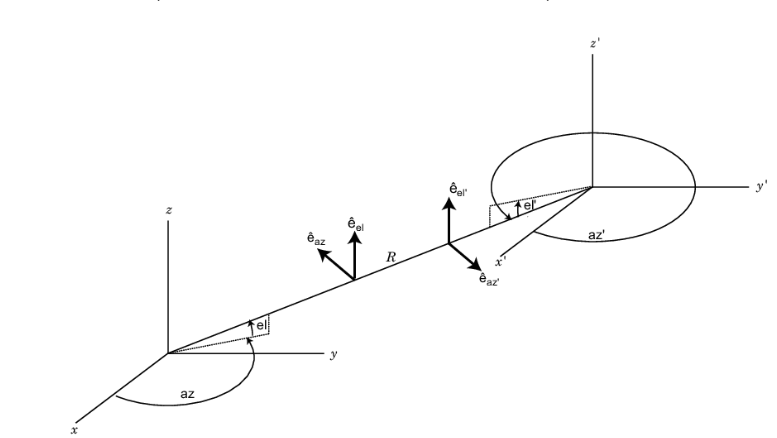
\includegraphics[width=3.22in,height=1.82in]{image5.png}
		\caption{\label{2Dpattern} Local coordinates systems of tranmitter's and receiver's antennas for polarization loss calculation \cite{balanis}}
	\end{center}
\end{figure}




\subsection{Link Budget}

 The link budget is a summary of the transmitted power considering all the gains and losses in the system and this enables the strength of the received signal to be estimated. The knowledge of the link budget is helpful for survey tools and measurements, because the expected values and the measured or observed value may differ from the originally transmitted or expected value. The link budget explains the values of the signal strength at the receiver input.

$\text{Received Power } \left( dBm \right) =Transmitted Power  \left( dBm \right) +Gains  \left( dB \right) -Losses  \left( dB \right)$

A typical link budget formula for radio communications is:

$P_{Rx}= P_{Tx~}+G_{Tx}+ G_{Rx}-L_{Tx}-L_{Rx}-L_{FSPL}-L_{P}$



Where $P_{Rx}$ is the received power in dBm, $P_{Tx}$ is the transmitter output power in dBm, $G_{Tx}$ and $G_{Rx}$ the transmitter and receiver antenna gain in dBi, $L_{Tx}$ and $L_{Rx}$ the transmit and receiver feeder losses, $L_{FSPL}$ the free space path loss in dB and $L_{P}$ describes the propagation losses including polarization mismatch, medium losses \ldots

\subsection{Bandwidth}

The bandwidth of an antenna is the range of frequencies over which the antenna can operate correctly, in other words the performance of the antenna conforms to some standard with respect to certain specified characteristics, such as input impedance, beam width, gain, radiation efficiency and beam direction which all should be within an acceptable value of that of the center frequency. The antenna’s bandwidth can also be described in terms of percentage of the center frequency $F_{C}$ of the band or a ratio between the upper and lower frequencies $F_{H}$  and $F_{L}$ for broadband antennas.

{\fontsize{12pt}{14.4pt}\selectfont $BW=100  \times \frac{F_{H}-F_{L}}{F_{C}} $}

\textbf{2.2.12 Diversity and Beamforming and max ratio combining }


\section{Measurement Uncertainty}

Measurement Uncertainty (MU) is a quantitative indication of measurement results quality which allows values comparison among the same measurement or to reference values. This work investigates the novel approach of normalized measurements, and compares it, in terms of accuracy to its conducted alternatives. For the sake of making the results of measurements of physical quantities easy to asses and evaluate with respect to its reliability, we need some indications so that measurement results can be compared, either among themselves or with respect to values specified in standards and this is what we refer to as measurement uncertainties. 

In this section the most used methodologies for the evaluation of measurement uncertainty are explained. There are two different types of MU evaluation: Type A which is defined as $``$the method of evaluation of uncertainty by the statistical analysis of series of observations$"$  (reference the Guide to the Expression of Uncertainty in Measurement).

The purpose of the Type A and Type B classification is to indicate the two different ways of evaluating uncertainty components and is for convenience of discussion only. Both types of evaluation are based on probability distributions and the uncertainty components are usually quantified by variances or standard deviations.

Evaluating type, A uncertainty is achieved using:

\begin{itemize}
	\item Arithmetic mean:  $\overline{x}=\frac{1}{n} \sum _{i=1}^{n}x_{i}$

	\item Standard deviation: $\sigma = \sqrt[]{\frac{1}{n-1} \sum _{i=1}^{n} \left( \overline{x}-x_{i} \right) ^{2}}$

	\item Standard uncertainty:

	\item Degrees of Freedom: $``$The number of values in the final calculation of a statistic that are free to vary$"$  with the form  $\vartheta =n-1$
\end{itemize}


Type B evaluation of uncertainty is defined as $``$the method of evaluation of uncertainty by means other than the statistical analysis of series of observations$"$ . Essentially, type B uncertainty is data collected from anything other than an experiment performed by you. For example, datasheets, white papers, industry guides, calibration reports or other available information.
